\chapter{Standing wave gate beams for coupling strength modulation}

In this chapter we will discuss experiments with standing wave laser fields and how the coupling strengths of carrier and sideband transitions may be controlled in our configuration. The results of this chapter were presented in Physical Review A \cite{StandingWave}.   

\section{Carrier and sideband coupling strengths in standing wave fields}

\begin{figure}[t]
    \begin{center}
        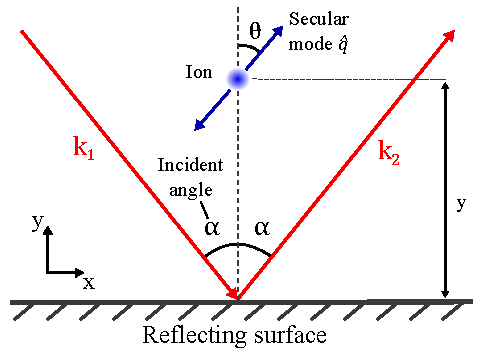
\includegraphics{figures/4/Fig_SWgeometry2}
        \caption{\label{fig:SWgeometry} Basic geometry of our standing wave configuration. An incident beam $\mathbf{k_1}$ at angle $\alpha$ w.r.t. surface normal is reflected, producing a second beam $\mathbf{k_2}$. The ion oscillates on a secular mode at angle $\theta$ w.r.t. the surface normal; its equilibrium height above the surface is $y$.   }
    \end{center}
\end{figure}

Here we will follow Sec. 2.3 and derive carrier and 1$^{st}$ order sideband coupling strengths for an ion interacting with two individual running-wave fields--one incident and one reflected from a nearby surface. Fig. \ref{fig:SWgeometry} illustrates the basic geometry in this situation. The incident and reflected beams $\mathbf{k_1}$ and $\mathbf{k_2}$ are each at an angle $\alpha$ with respect to the surface normal, and $|k_1| = |k_2| = k$. The ion's secular mode of interest oscillates with frequency $\omega$ at an angle $\theta$ with respect to the surface normal. The ion's mean height above the reflecting surface is given by $y$. For simplicity we will assume that the incident beam and secular axis are coplanar. 

The ion's motion in the $xy$ plane is described with the position operators $\hat{x}' = \hat{x}$ and $\hat{y}' = y + \hat{y}$. If $\hat{q}$ is the position operator corresponding to the ion's secular axis, then we have
\begin{equation}
\begin{split}
\hat{x}' &= \hat{q} \sin \theta \\
\hat{y}' &= y + \hat{q} \cos \theta \text{.}
\end{split}
\end{equation}
The ion's Hamiltonian per Eq. \ref{eq:basicH} will contain a term $\hat{H}_i$ for each beam:
\begin{equation}
\begin{split}
\hat{H}&_{i,1} = \frac{1}{2} \hbar \Omega_1 (\sigma_+ + \sigma_-) ( e^{i (\mathbf{k_1} \cdot \mathbf{\hat{r}} } e^{-i (\nu t - \phi)} + e^{-i (\mathbf{k_1} \cdot \mathbf{\hat{r}} } e^{i (\nu t - \phi)} ) \\
\hat{H}&_{i,2} = \frac{1}{2} \hbar \Omega_2 (\sigma_+ + \sigma_-) ( e^{i (\mathbf{k_2} \cdot \mathbf{\hat{r}} } e^{-i (\nu t - \phi)} + e^{-i (\mathbf{k_2} \cdot \mathbf{\hat{r}} } e^{i (\nu t - \phi)} ) \\
\hat{H}&_i = \hat{H}_{i,1} + \hat{H}_{i,2}  \text{,}
\end{split}
\label{eq:His}
\end{equation}  
where $\Omega_1$ and $\Omega_2$ are the respective coupling strengths in each interaction. The different coupling strengths arise from the differences in field strength between the two beams at the ion's position--this can be due to imperfect reflectivity from the surface, scattering of the reflected beam from surface features, varying intensities in the Gaussian beam shapes, or some combination thereof. The terms $\mathbf{k_1} \cdot \mathbf{\hat{r}}$ and $\mathbf{k_2} \cdot \mathbf{\hat{r}}$ in $H_i$ can be expressed as 
\begin{equation}
\begin{split}
\mathbf{k_1} \cdot \mathbf{\hat{r}} =& \ k \cos \alpha (-\hat{y}') + k \sin \alpha (\hat{x}') \\
=& -k y \cos \alpha + [ \sin \theta \sin \alpha - \cos \theta \cos \alpha ] k \hat{q} \\
\mathbf{k_2} \cdot \mathbf{\hat{r}} =& \ k \cos \alpha (\hat{y}') + k \sin \alpha (\hat{x}') \\
=& \ k y \cos \alpha + [ \sin \theta \sin \alpha + \cos \theta \cos \alpha ] k \hat{q} \text{.}
\end{split}
\label{eq:kdotr}
\end{equation}

Transforming now into the interaction picture $\hat{H}_I = \hat{U}_0^{\Dagger} \hat{H} \hat{U}_0$ as before, and making the substitutions in Eq. \ref{eq:kdotr} as well as $\gamma =( k y \cos \alpha )$ and $\hat{q} = \sqrt{\hbar / (2 m \omega)} (\hat{a} + \hat{a}^{\dagger})$, we obtain 
\begin{equation}
\begin{split}
\hat{H}_I = \frac{\hbar}{2} \hat{\sigma}_+ e^{-i (\Delta t - \phi) } \bigg\{& \ \Omega_1 \text{exp} \big[ -i \gamma + i \eta_1 ( \hat{a}(t) + \hat{a}^{\dagger}(t) ) \ \big] \\ 
+& \ \Omega_2 \text{exp} \big[ \ i \gamma + i \eta_2 ( \hat{a}(t) + \hat{a}^{\dagger}(t) ) \ \big] \bigg\} + \text{H.c.} \text{,}
\end{split}
\label{eq:HintSW}
\end{equation}
where $\eta_1$ and $\eta_2$ define respective Lamb-Dicke factors for each of the two beams:
\begin{equation}
\begin{split}
\eta_1 &= k \sqrt{ \frac{\hbar}{2 m w} }  [ \sin \theta \sin \alpha - \cos \theta \cos \alpha ] \\
\eta_2 &= k \sqrt{ \frac{\hbar}{2 m w} }  [ \sin \theta \sin \alpha + \cos \theta \cos \alpha ] \text{.}
\end{split}
\label{eq:etaSW}
\end{equation}
The coupling strength for the $|g,n\rangle \leftrightarrow |e,n+m\rangle$ transition becomes
\begin{equation}
\begin{split}
\Omega_{n+m, n} =& \ \Omega_1 e^{-i \gamma} \langle n + m | e^{ i \eta_1 ( \hat{a}(t) + \hat{a}^{\dagger}(t) ) } | n \rangle \\
+& \ \Omega_2 e^{i \gamma} \langle n + m | e^{ i \eta_2 ( \hat{a}(t) + \hat{a}^{\dagger}(t) ) } | n \rangle 
\label{eq:swRabiFreq}
\end{split}
\end{equation}
Making the Lamb-Dicke regime approximation once again, we can now find definitions for the carrier and sideband coupling strengths in the two-beam configuration:
\begin{equation}
\begin{split}
\Omega_{car} = \ &\Omega_1 e^{-i \gamma} \bigg[1 - \frac{\eta_1^2}{2}(1 + 2n) \bigg] + \Omega_2 e^{i \gamma} \bigg[1 - \frac{\eta_2^2}{2}(1 + 2n) \bigg] 
\label{eq:OmegaCarSW}
\end{split}
\end{equation}
and
\begin{equation}
\begin{split}
\Omega_{rsb} &= \sqrt{n} \ \big( \Omega_1 e^{-i \gamma} \eta_1 + \Omega_2 e^{i \gamma} \eta_2 \big) \\
\Omega_{bsb} &= \sqrt{n+1} \ \big( \Omega_1 e^{-i \gamma} \eta_1 + \Omega_2 e^{i \gamma} \eta_2 \big) \\ \text{.}
\end{split}
\label{eq:OmegaSbSW}
\end{equation}

Interference between the $e^{\pm i \gamma}$ terms produces fringes in the coupling strengths as the ion's equilibrium position $y$ changes. When $\cos \theta \cos \alpha > \sin \theta \sin \alpha$, $\eta_1$ and $\eta_2$ have opposite sign, and the carrier and sideband fringes are 180$^o$ out of phase. The $\gamma = k y \cos \alpha$ term represents the optical phase of the standing wave field which results from the mixing of beam components $k_{1,y} = - k \cos \alpha$, $k_{2,y} = k \cos \alpha$. When the ion's position coincides with a node of the standing wave, $\gamma = l \pi$ (with $l$ an integer), and $\Omega_{car}$ is maximized while $\Omega_{rsb}$ and $\Omega_{bsb}$ are minimized. On an antinode, $\gamma = (l + 1/2) \pi$, and the converse is true. In between the nodes and antinodes there will be a mixture of both carrier and sideband coupling. This node/antinode behavior refers to the case of a quadrupole transition; the behavior will be reversed for a dipole transition.

Achieving complete suppression requires $\Omega_1 = \Omega_2$ and $\alpha = 0$. If $\Omega_1 \neq \Omega_2$, then the field strengths $E_0$ of the incident and reflected beams are unequal at the ion's position, leading to some amount of residual running-wave light in the $y$ direction that will excite the ion indifferently. If $\alpha \neq 0$ then the same thing occurs, with the residual light propagating parallel to the trap surface in this case. \footnote{It is possible to completely suppress just the sidebands in the $\alpha \neq 0$ case, provided that the plane of the incident/reflected beams is orthogonal to the plane of the ion's oscillation axis, or alternatively if $\theta = 0$.}  


%%%%%%%%%%%%%%%%%%%%%%%%%%%%%%%%%
\section{Experimental realization}

\begin{figure}[t]
    \begin{center}
        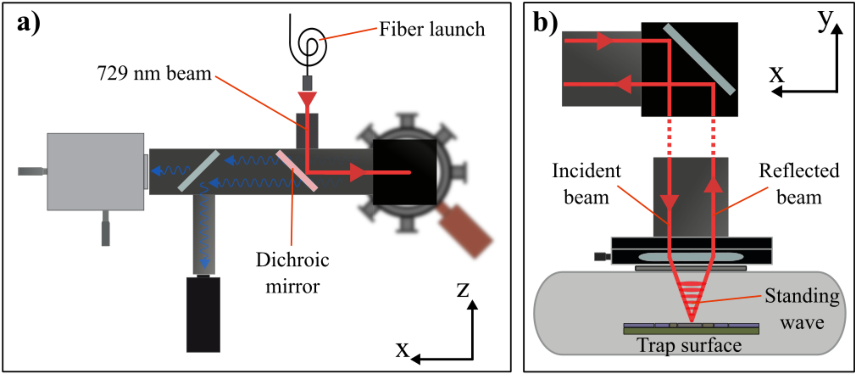
\includegraphics{figures/4/Fig_SWlaserConfigR}
        \caption{\label{fig:SWlaserConfig} (a) Top-down and (b) side-on views of the 729 nm laser configuration in this experiment. To achieve normal incidence of a 729 beam onto our trap surface, we use a dichroic mirror to introduce the beam into the optical path of our camera and PMT (see Sec. 3.3 and Fig. \ref{fig:CameraConfig}). By steering the incident beam and viewing the reflected beam's return path, we have minimized the incident angle depicted in (b) as much as possible.    }
    \end{center}
\end{figure}


The Gen IIc trap has a patterned aluminum surface which reflects 729 nm light with an 86\% reflectivity. We can therefore use the trap surface itself as the reflecting mirror for a standing wave field. This has the advantage of requiring no additional optics, save for those which steer the incident beam. As an added advantage, the ''mirror'' in this scenario will always remain a constant distance away from the ion, eliminating any concern of phase fluctuations in the field arising from microscopic movements of the mirror. Using a dichroic filter, we introduced a 729 nm beam into the optical path of the CCD camera and detection PMT in our setup. Fig. \ref{fig:SWlaserConfig} illustrates the configuration. Upon passing through the focusing lens for the camera/PMT (Fig. \ref{fig:SWlaserConfig} (b)), the beam is incident on the trap surface at an angle $\alpha \approx 20^o$. By steering the incident beam and viewing the reflected beam on its return path we were able to minimize this angle to the best of our ability. 

We excited ions on the $|S_{1/2}, m_J = -\frac{1}{2} \rangle \rightarrow |D_{5/2}, m_J = -\frac{5}{2} \rangle$ carrier transition in this experiment. Sideband excitations were performed on the radial mode with $\nu=2\pi \times 4.75$ MHz (on the RF null) and $\theta = 13^{\circ}$. Doppler cooling was done before every interaction, whereas sideband cooling was withheld in order to preserve enough quanta for appreciable sideband coupling strengths. To displace an ion's equilibrium position along the standing wave axis, we apply a static offset field $E_y$ through suitable adjustments to the trap's waveforms and potentials, as described in Sec. 3.1. The case $E_y$ = 0 corresponds to the ion being on the RF null. For $E_y>0$ and $E_y<0$, the ion is displaced along $+y$ and $-y$, respectively. The range of $E_y$ values used in this experiment displaces the ion over a 10 $\mu$m range. %The fringes in the carrier and sideband transitions resulting from this displacement are evident in Fig.~\ref{fig:EyScan}.

Displacing the ion from its equilibrium position on the RF null introduces micromotion, which will affect the dynamics in several ways beyond the coupling strength fringing. First, there will be an additional modulation to both the carrier and sideband coupling strengths \cite{Berkeland98.JAP.83.5025}. To account for this modulation, we multiply Eqs. \ref{eq:OmegaCarSW} and \ref{eq:OmegaSbSW} by the Bessel function $J_0(\kappa)$, where $\kappa$ is the modulation parameter given by
\begin{equation}
\label{eq:kappa}
\kappa = \cos \beta \frac{2}{\lambda\, \Omega_{RF}} \sqrt{ \frac{V_{pp}(x,y)}{m}  } .
\end{equation}
Here $\lambda = 729$ nm, $V_{pp}(x,y)$ is the RF pseudopotential, and $\beta$ is the angle between the micromotion direction and the standing wave axis.  Second, the ion's secular frequencies change depending on its position within the RF field. We account for this simply by measuring the sideband resonance at various displacements and parameterizing the results.

We can minimize micromotion in the $x$ direction by applying a static field $E_x$, suitably proportional to $E_y$, in order to displace the ion an angle which is twice that of the RF quadrupole axis. Along this trajectory the ion will experience only vertical RF field vectors (see Fig. \ref{fig:quadrupole}). Restricting the micromotion to the $y$ dimension is equivalent to choosing $\beta = 0$ in Eq. \ref{eq:kappa}.

\begin{figure}[t]
    \begin{center}
        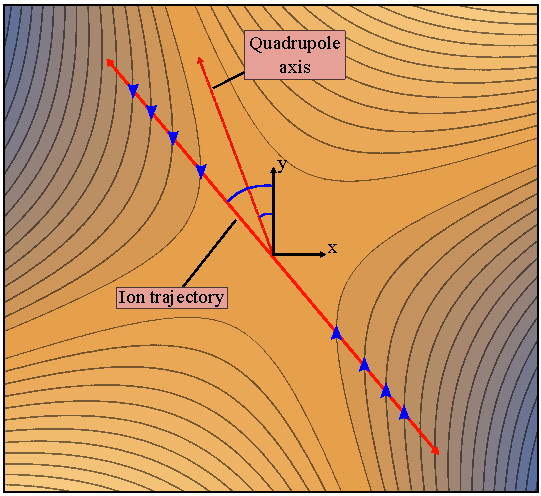
\includegraphics{figures/4/Fig_Quadrupole}
        \caption{\label{fig:quadrupole} Illustration of field vectors in a rotated quadrupole field. By displacing the ion at an angle which is twice that of the quadrupole axis, it will encounter field vectors that are only in the $\pm y$ direction (blue arrows). As such, horizontal micromotion will be minimized.  }
    \end{center}
\end{figure}






%%%%%%%%%%%%%%%%%%%%%%%%%%%%%%%%%
\section{Results}


\subsection{Coupling strength fringing and suppression}


\begin{figure*}
    \begin{center}
        %\makebox[\textwidth][c]{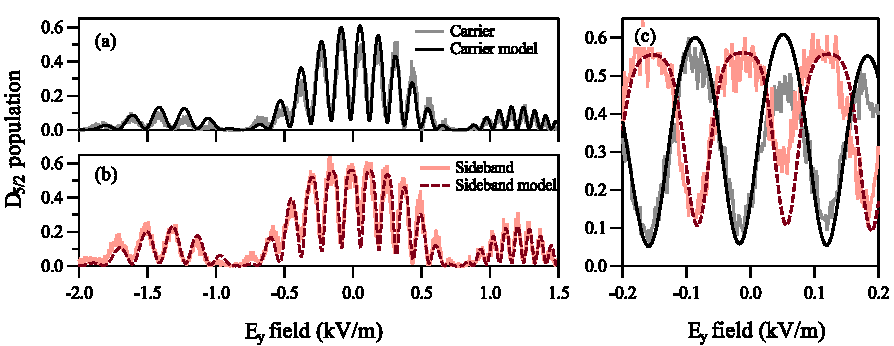
\includegraphics[width=1.2\textwidth]{figures/4/Fig_fringes3}}
        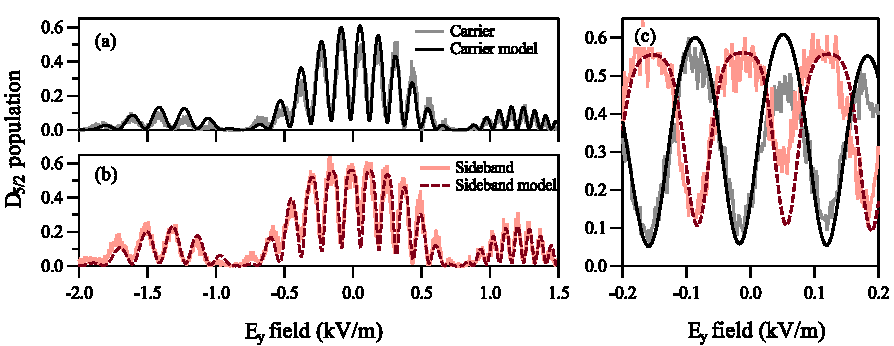
\includegraphics{figures/4/Fig_fringes3}
        \caption{\label{fig:fringes} $D_{5/2}$ populations vs. applied $E_y$ field measured after (a) carrier and (b) red sideband transitions. The sideband's gate beam power is 9.5~dB greater than the carrier's, and the interaction time is fixed for both cases (13~$\mu$s).  The overall envelope is generated by the micromotion modulation $J_0(\kappa)$ (see text). (c) The carrier and sideband populations oscillate 180$^o$ out of phase as the ion is transported through the standing wave fringes. The solid lines represent a fit to the data using the model described in the text. The deviation between the data and fit at $E_y\approx0.05$~kV$/$m may be due to scattering of the reflected light from the trap surface.}
    \end{center}
\end{figure*} 



Figs. \ref{fig:fringes} (a) and (b) show $D_{5/2}$ state populations measured after driving carrier or red sideband transitions as a function of applied $E_y$ field. The laser interaction time was fixed for all excitations (13 $\mu$s), and the power was set 9.5 dB greater for the sideband interactions in order to achieve an approximately equal population inversion. As can be seen in Fig. \ref{fig:fringes}, we observe the predicted fringing due to the standing wave field's phase, which are superimposed with the $J_0(\kappa)$ envelope resulting from micromotion modulation. Per Eqs. \ref{eq:OmegaCarSW} and \ref{eq:OmegaSbSW}, the maxima of the carrier fringes correspond to the ion positioned on nodes of the standing wave, whereas the minima correspond to antinodes. The carrier and sideband fringes are overlaid in Fig. \ref{fig:fringes} (c), demonstrating the 180$^{\circ}$ phase difference which occurs when the condition $\cos \theta \cos \alpha > \sin \theta \sin \alpha$ is met.



\begin{figure}[tbh]
    \begin{center}
        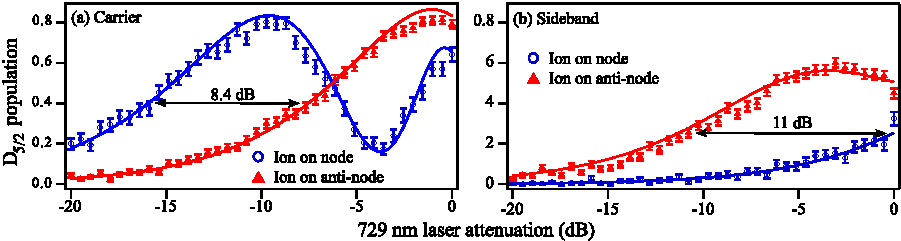
\includegraphics{figures/4/Fig_powerdb}
        \caption{\label{fig:PowerScans} $D_{5/2}$ populations vs. relative laser beam power measured after (a) carrier and (b) red sideband transitions. Interaction time is fixed for both cases (13~$\mu$s). The populations were measured with the ion on either a node (blue circles, $E_y = -0.08$ kV/m) or an adjacent anti-node (red triangles, $E_y = -0.01$ kV/m) near the RF null ($J_0(\kappa) \approx 1$). An effective suppression of 8.4 dB for the carrier and 11 dB for the sideband is achieved. The solid lines represent a simultaneous fit to the data using the model described in the text. For reference, the results from Fig.~\ref{fig:fringes} (a) and (b) were acquired at -13.5 dB and -4 dB, respectively.}
    \end{center}
\end{figure}

In Fig. \ref{fig:PowerScans} we measured $D_{5/2}$ populations after driving the carrier and red sideband transitions as a function of applied laser power. The interaction time was once again fixed (13 $\mu$s, as before). We performed this experiment with the ion on both a standing wave node and antinode, using the results in Fig. \ref{fig:fringes} to select appropriate displacement fields $E_y$. Choosing a node and antinode close to the RF null minimized the micromotion modulation. By measuring the separation between the node and antinode curves, we are able determine the amount of carrier and sideband suppression achieved in our setup. For the carrier, the suppression is equivalent to an 8.4 dB reduction in driving laser power. For the sideband, and equivalent 11 dB reduction can be achieved. 



\subsection{Data fits}

To produce the fits seen in Figs. \ref{fig:fringes} and \ref{fig:PowerScans}, we use Eq. \ref{eq:Pe} to calculate $P_e(t)$ in the case of $\delta = 0$:
\begin{equation}
P_e(t) = \mathlarger{\sum_{n=0}^{\infty}} P_n (\bar{n}) \sin^2 \bigg[ \frac{1}{2} \ J_0(\kappa) \ \Omega_{car/rsb}(\gamma, n) \ t \bigg] \text{,}
\end{equation}
where the coupling strengths are those from Eqs. \ref{eq:OmegaCarSW} or \ref{eq:OmegaSbSW}, respectively. We parameterize a simultaneous fit with 
\begin{equation}
\kappa^2 = \sum_{j=2}^{4} m_j E_y^j
\end{equation}
for the micromotion parameter, and 
\begin{equation}
y = \sum_{j=0}^{4} a_j E_y^j
\end{equation}
for $\gamma = k y \cos \alpha$ , with $m_j$ and $a_j$ the respective fit coefficients. These coefficients, along with $\Omega_1$, $\Omega_2$, $\alpha$, and $\bar{n}$ form the complete set of parameters that defines the simultaneous fits in Figs. \ref{fig:fringes} and \ref{fig:PowerScans}. In particular, we have in this case $|\alpha| = 18^o$, $\Omega_2 / \Omega_1 = 0.52$, and $\bar{n} = 18$. The deviation between the data and the fit near $E_y \approx 0.05$ kV/m in Fig. \ref{fig:fringes} (c) may be due to interactions with light scattered from the trap surface. Otherwise, we see no other significant deviations. The values of $\alpha$ and $\Omega_2 / \Omega_1$ are consistent with the incomplete suppression we measure for the carrier and sideband. 



\subsection{Comparison with numerical models}

Using both the experimental and fitting data we have compared our results to those from a numerical model of our trapping potentials. From the fringe data in Fig. \ref{fig:fringes} we can infer the ion's displacement $y$ as a function of $E_y$ (since fringe maxima corresponds to half a wavelength). From $\kappa^2$ we can determine the pseudopotential $V_{pp}$ as a function of $E_y$ as well. Fig. \ref{fig:model} plots $y(E_y)$ and $V_{pp}(E_y)$ along with their respective predictions from the model. We see good agreement between the respective data sets, providing a measure of confidence in the model for future use. The model includes a 700 V/m uniform stray field that was adjusted to match the observed RF null in Fig. \ref{fig:fringes}. Also. the magnitude of the RF potential in the model was adjusted to match the observed mode frequency at $E_y = 0$. Otherwise, there are no other free parameters used in the model. 

\begin{figure}[htb]
    \begin{center}
        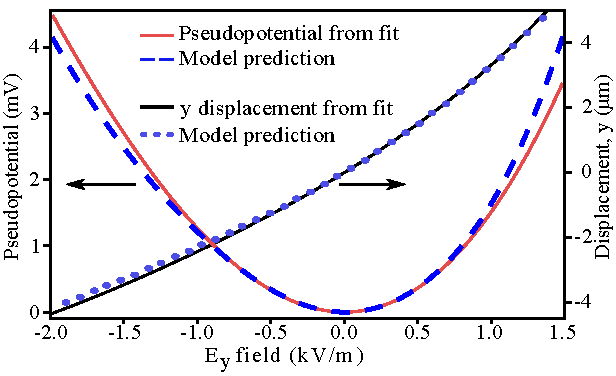
\includegraphics{figures/4/Fig_PPfit}
        \caption{\label{fig:model} Dependence of the pseudopotential $V_{pp}$ and ion displacement $y$ on the applied field $E_y$, along with predictions from a numerical model of the trapping potentials. Deviations from the model can be attributed non-uniformity of the stray fields in the trapping region. }
    \end{center}
\end{figure}




%%%%%%%%%%%%%%%%%%%%%%%%%%%%%%%%
\section{Discussion}

As discussed in Sec. 4.1, the degree of carrier and sideband suppression achievable ultimately depends on the quality of the standing wave field at the ion's position, which, aside from the incident angle $\alpha$, is related to the ratio $\Omega_2\, / \, \Omega_1$. The value $\Omega_2 / \Omega_1 = 0.52$ in our experiment suggests either spacial misalignments in the incident and reflected beams, scattering of the reflected beam from the trap's surface features, or some combination thereof. The Gen IIc trap's surface reflectivity places a limit on $\Omega_2\, / \, \Omega_1=\sqrt{0.86}=0.93$. Approaching this limit would allow for a carrier suppression equivalent to a 29 dB reduction in laser power when $\bar{n}\approx0$ and $|\alpha|<10^{\circ}$. Further carrier suppression would require the use of a different trap with a more reflective surface. For instance, we measure the reflectivity from a gold coated trap like the one described Ref. \cite{Guise15.JAP.117.174901} to be $>98\%$, which could provide an equivalent carrier suppression of $>\,$40 dB. Similar quality standing waves could be generated by incorporating a metallic mirror adjacent to an ion trap--however, phase fluctuations in the standing wave field could become an issue in such a configuration.

Suppression of the carrier implies that the driving laser's power may be freely increased by an amount equivalent to the effective suppression, allowing for faster sideband interactions with no increased chance of an off-resonant carrier excitation. For the 8.4 dB effective carrier suppression we achieve, sideband interactions could be performed 2.5 times faster; at the 29 dB suppression limit of our aluminum trap, 28 times faster; at the $>\,$40 dB suppression limit of a gold coated trap, $>\,$100 times faster.